\section{Synthetic demo: refocusing Blender scenes with known optics}\label{sec:blender}
\textbf{Motivation.} The real dataset has no ground-truth optics. For a demo we built depth-layered scenes in Blender 4.5 (Cycles, thin-lens depth of field, 640$\times$896, 48 samples with denoising) from public-domain (CC0) Poly Haven\footnote{\url{https://polyhaven.com}} models (rubber duck, apple, marble bust, potted plant, concrete cat statue, rocks, tree) and HDRI lighting (\texttt{studio\_small\_09}, \texttt{kloofendal\_48d\_partly\_cloudy\_puresky}). For each scene we render a true 9-frame focal stack by moving the camera's focus distance, give \emph{one} frame to the authors' released model, and compare its generated stack with the rendered one. We measure local sharpness (variance of the Laplacian) in a box around each object for every frame. \textbf{Important limitations:} the mapping from the phone's lens positions 0--8 to focus distances is not given, so every mapping below is our assumption; the renders are synthetic, so a domain shift from smartphone photos is unavoidable; and each result is one scene, one input frame, one sample.

\textbf{Experiment 1: full-frame-style camera, f/1.4, distances 0.45--200\,m (guessed log spacing).} In thumbnails the model's stack looked nearly static. Measuring sharpness per object shows it \emph{does} sweep focus in near-to-far order, but its peaks are misplaced: for the bust the correlation between the ground-truth and model sharpness curves is $-0.14$, for the cat $0.20$ (input at position 2).

\textbf{Experiment 2: weaker blur.} Rendering the same scene at f/4 raised the correlations to duck $0.32$, bust $0.46$ and cat $0.81$ (Figure~\ref{fig:sharp}), consistent with, but not proof of, the idea that our first renders had far more blur than smartphone photos. At f/8 even the ground-truth stack barely changes across positions, so that setting is uninformative.
\begin{figure}[h]\centering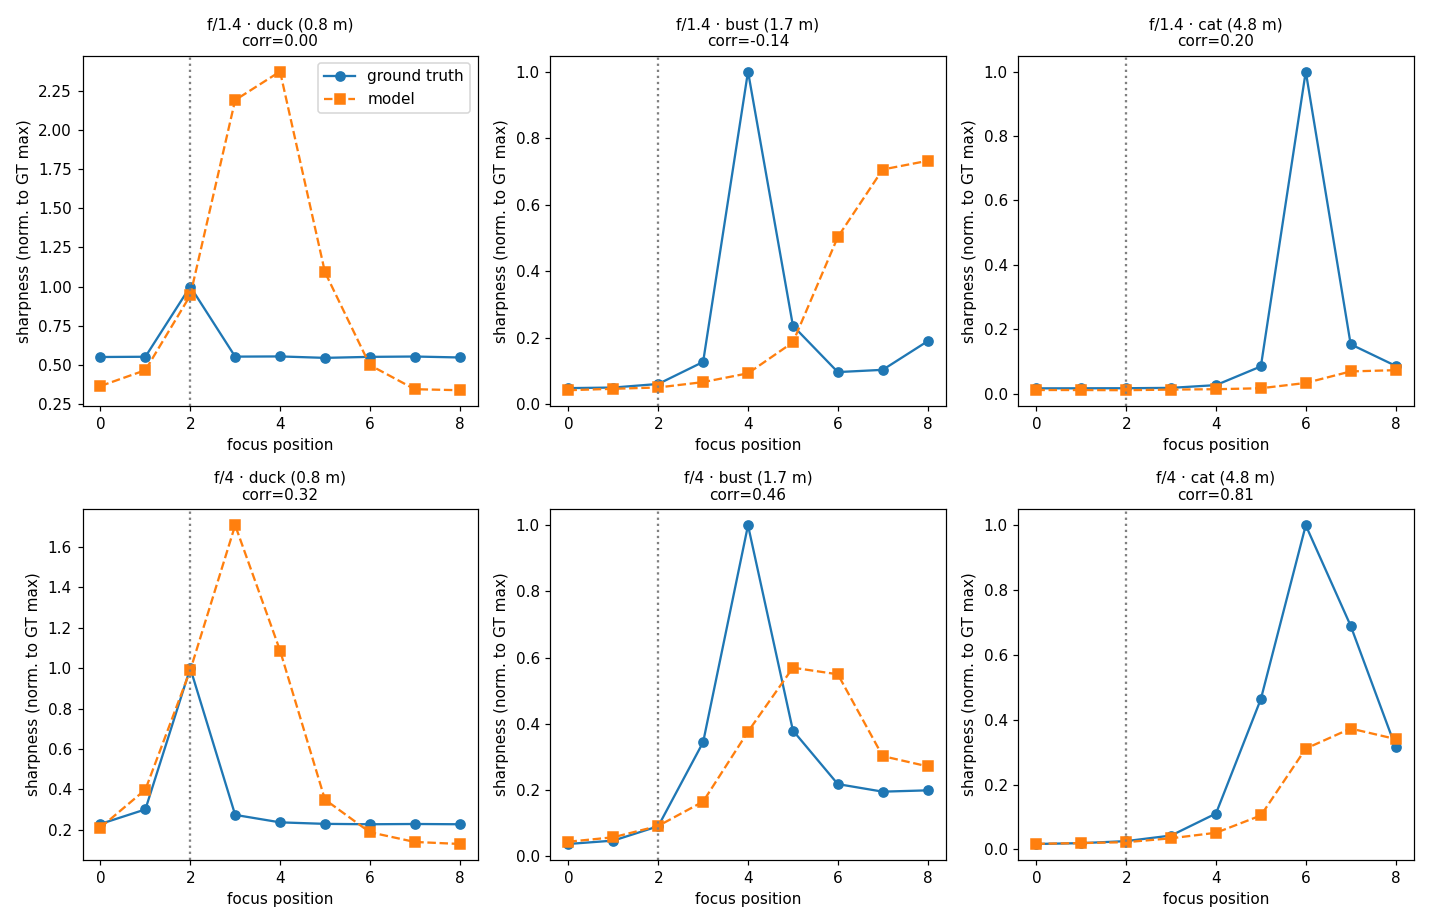
\includegraphics[width=\linewidth]{sharp_curves.png}
\caption{Sharpness per focus position at three objects, ground truth vs model (input at position 2, vertical dotted line). Top: f/1.4. Bottom: f/4.}\label{fig:sharp}\end{figure}

\textbf{Experiment 3: phone-like macro scene.} The repository README says positions 0--8 correspond to lens positions 0--0.8, i.e.\ 5\,cm to infinity. \emph{Assuming} the spacing is linear in diopters, positions 4, 5, 6, 7 correspond to 10, 13.3, 20 and 40\,cm. We therefore rebuilt the scene at that scale (objects at 0.10, 0.133, 0.20 and 0.40\,m, camera with a 7\,mm sensor, 6\,mm lens, f/1.8), so that by construction the duck, apple, bust and cat are sharpest at positions 4, 5, 6 and 7. The duck's measurement box is dominated by background texture (its ground-truth curve has two peaks), so we discard the duck.
\begin{table}[h]\centering
\caption{Macro scene: sharpness-peak position, ground truth vs model (authors' checkpoint). ``Shift'' = model peak $-$ ground-truth peak.}\label{tab:macro}
\begin{tabular}{lccccc}\toprule
Input position & Object & GT peak & Model peak & Shift & Curve corr.\\\midrule
4 & apple & 5 & 6 & $+1$ & 0.47\\
4 & bust & 6 & 7 & $+1$ & 0.33\\
4 & cat & 7 & 8 & $+1$ & 0.67\\
6 & apple & 5 & 3 & $-2$ & 0.04\\
6 & bust & 6 & 5 & $-1$ & 0.50\\
6 & cat & 7 & 4 & $-3$ & $-0.29$\\
\bottomrule\end{tabular}\end{table}
With the input at position 4 the model's apple, bust and cat sharpen in the right order but consistently one position late (Figure~\ref{fig:macro}). With the input at position 6 the peaks fall \emph{early} and are no longer in depth order. So the macro-scale assumption did \textbf{not} remove the offset, and the offset changes sign with the input position: the model's behaviour on synthetic scenes is not a fixed calibration error that a different distance mapping would fix.
\begin{figure}[h]\centering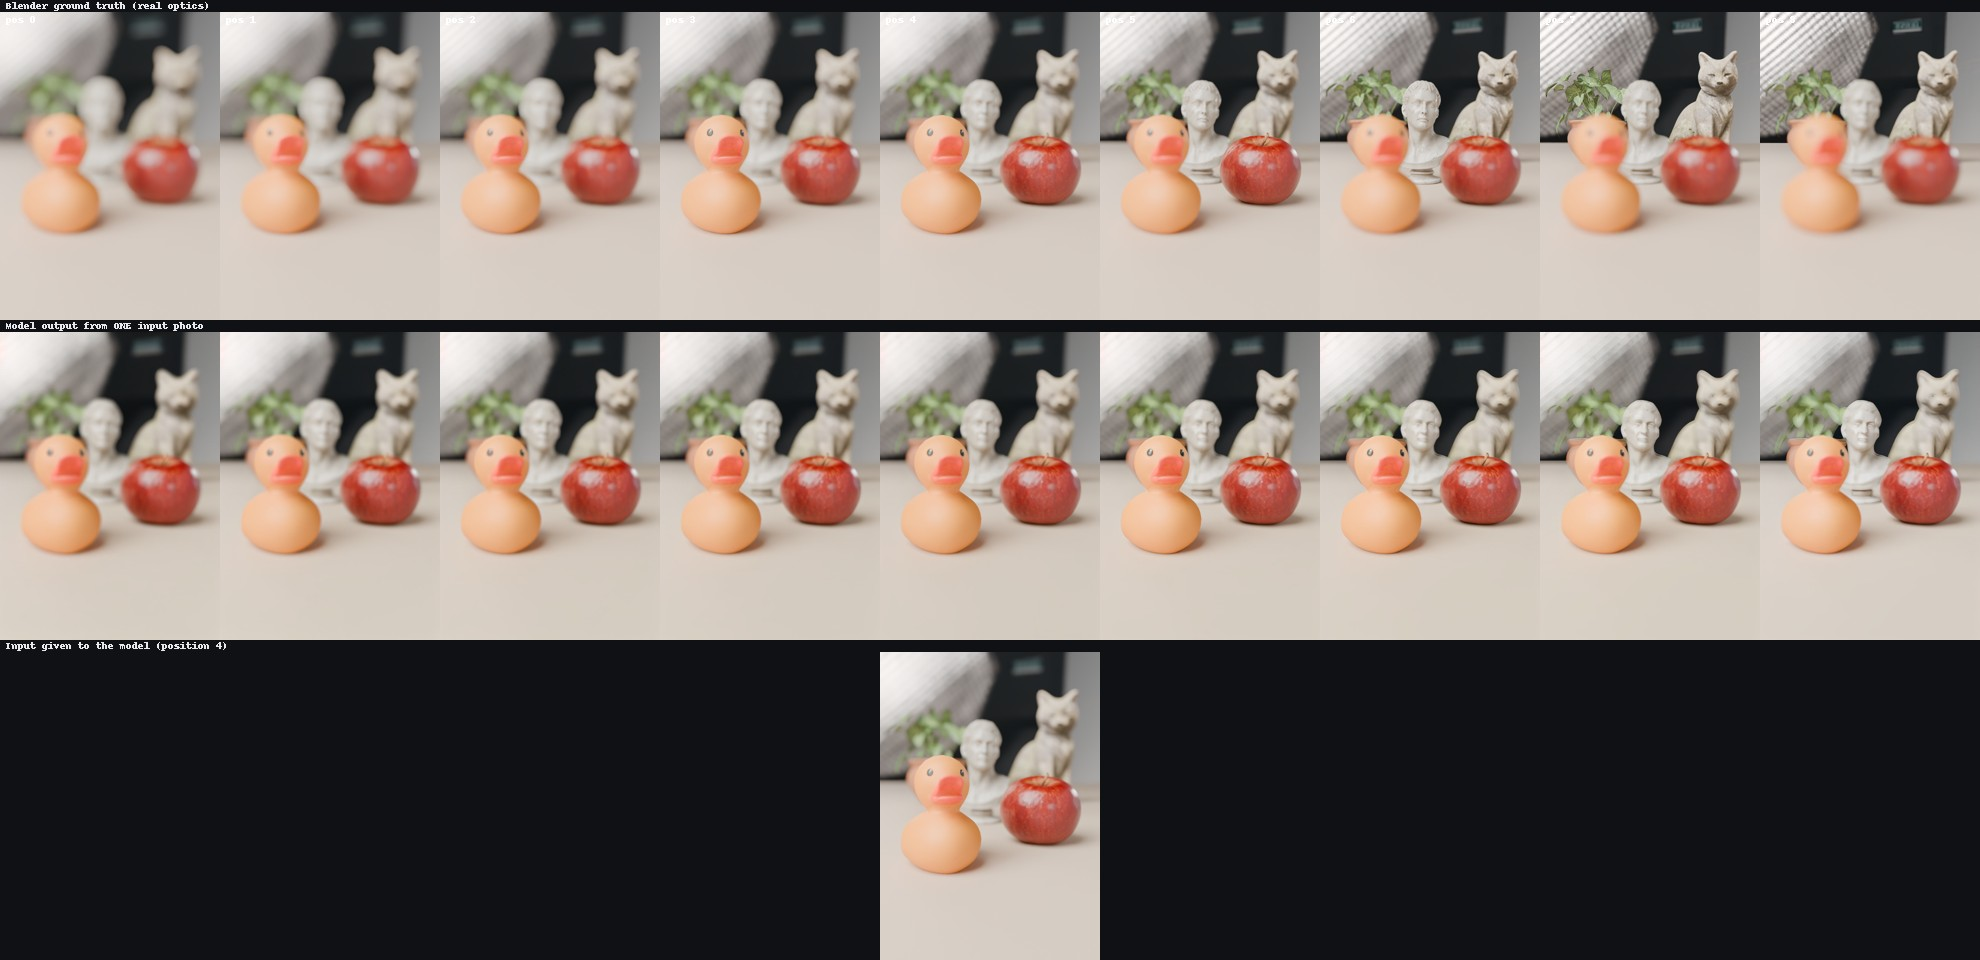
\includegraphics[width=\linewidth]{compare_macro_in4.jpg}
\caption{Macro scene, input at position 4. Top: ground-truth stack (Blender). Middle: authors' model output from the single input photo (bottom, position 4).}\label{fig:macro}\end{figure}

\textbf{Takeaway.} On synthetic scenes the released model produces a plausible near-to-far focus sweep but with a position error of one to three steps, and that error depends on the input position. We cannot separate a wrong distance-to-position assumption from the synthetic-to-real domain shift with this data; doing so would need real photos with known focus distances. For the live demo we therefore treat the Blender result as an illustration, not a benchmark.

